\section{Results}

\subsection{Primary Finding: Corpus-Quality Hypothesis Refuted}

At $\sim$300B training tokens, OLMo-7B does not achieve a higher MMLU/HellaSwag generalization balance ratio than Pythia-6.9B. The direction of the difference is reversed: Pythia achieves a higher ratio (0.565 vs.\ 0.538), and the 95\% bootstrap confidence interval lies entirely below zero, providing strong statistical evidence against the hypothesis.

\begin{table}[h]
\centering
\caption{Benchmark scores for Pythia-6.9B and OLMo-7B at $\sim$300B training tokens.}
\begin{tabular}{lllll}
\toprule
Model & MMLU & HellaSwag & ARC-Easy & ARC-Challenge \\
\midrule
Pythia-6.9B & 0.2588 & 0.4580 & 0.5861 & 0.2841 \\
OLMo-7B     & 0.2464 & 0.4580 & 0.6527 & 0.3388 \\
\bottomrule
\end{tabular}
\end{table}

\subsection{Primary Metric: MMLU/HellaSwag Generalization Balance Ratio}

\begin{table}[h]
\centering
\caption{Primary metric summary: MMLU/HellaSwag ratio and statistical analysis.}
\begin{tabular}{lllll}
\toprule
Model & Ratio & Difference & 95\% CI & Cohen's $d$ \\
\midrule
Pythia-6.9B & 0.565 & \multirow{2}{*}{$-0.0265$} & \multirow{2}{*}{$[-0.045, -0.007]$} & \multirow{2}{*}{$-2.732$} \\
OLMo-7B     & 0.538 & & & \\
\bottomrule
\end{tabular}
\end{table}

The ratio difference (OLMo $-$ Pythia) is $-0.0265$. The 95\% bootstrap CI $[-0.045, -0.007]$ lies entirely below zero, rejecting $H_0: R_{\text{OLMo}} \geq R_{\text{Pythia}}$. Cohen's $d = -2.732$ indicates a large effect size by conventional thresholds, though this magnitude is inflated by the small variance of per-subject MMLU estimates at 500-sample evaluation.

\begin{figure}[h]
\centering
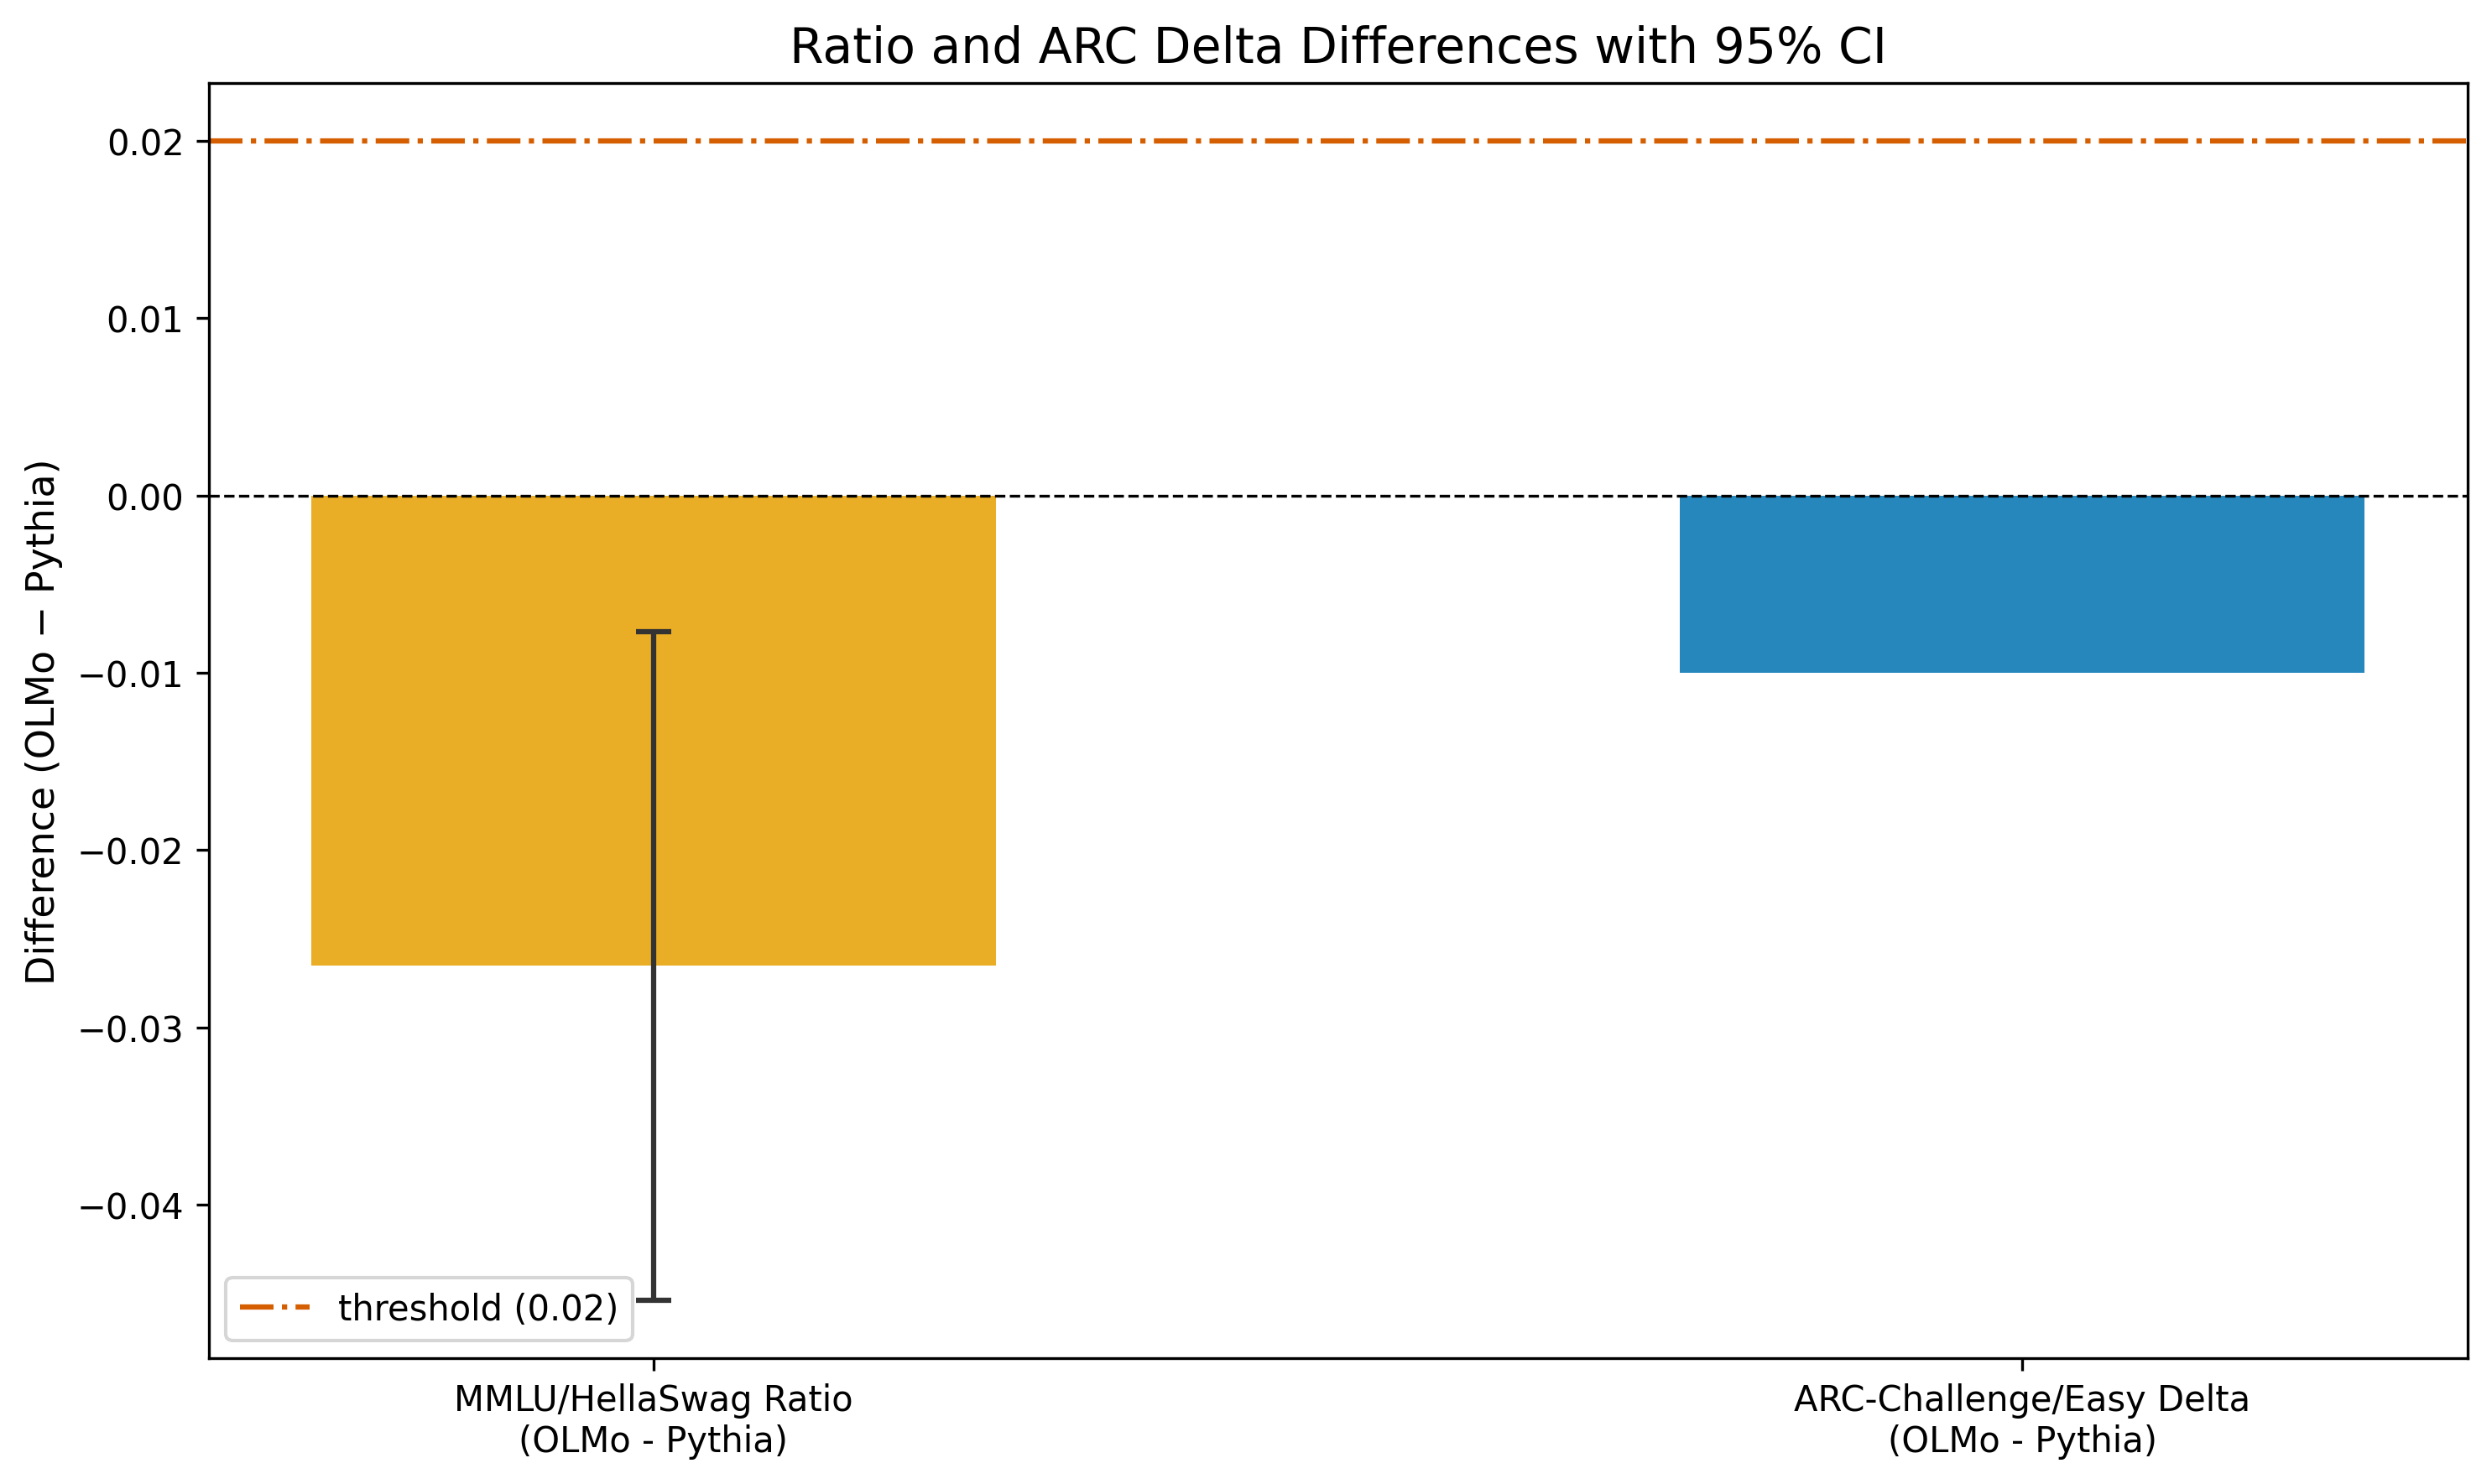
\includegraphics[width=0.48\textwidth]{figures/ratio_delta.png}
\caption{MMLU/HellaSwag ratio comparison with 95\% bootstrap CI. Pythia ratio $= 0.565$; OLMo ratio $= 0.538$; difference $= -0.0265$. CI $[-0.045, -0.007]$ lies entirely below zero.}
\label{fig:ratio}
\end{figure}

\subsection{Secondary Metric: ARC-Challenge/Easy Delta}

OLMo-7B achieves higher absolute scores on both ARC splits (ARC-Easy: 0.6527 vs.\ 0.5861; ARC-Challenge: 0.3388 vs.\ 0.2841). The difficulty delta is $\Delta_{\text{ARC}} = -0.3139$ for OLMo and $\Delta_{\text{ARC}} = -0.3020$ for Pythia. The difference in deltas ($-0.012$) is small and in the direction of slightly greater difficulty sensitivity for OLMo. This secondary result does not support a clear corpus quality signal: OLMo's higher ARC scores are consistent with architectural advantages (SwiGLU activations, different tokenizer) rather than corpus quality effects.

\subsection{Analysis: HellaSwag Convergence as a Structural Finding}

The most structurally informative result is that both models achieve identical HellaSwag scores (0.4580 each) to four decimal places. This is not a near-tie --- it is exact convergence at the precision of 500-sample evaluation.

\begin{figure}[h]
\centering
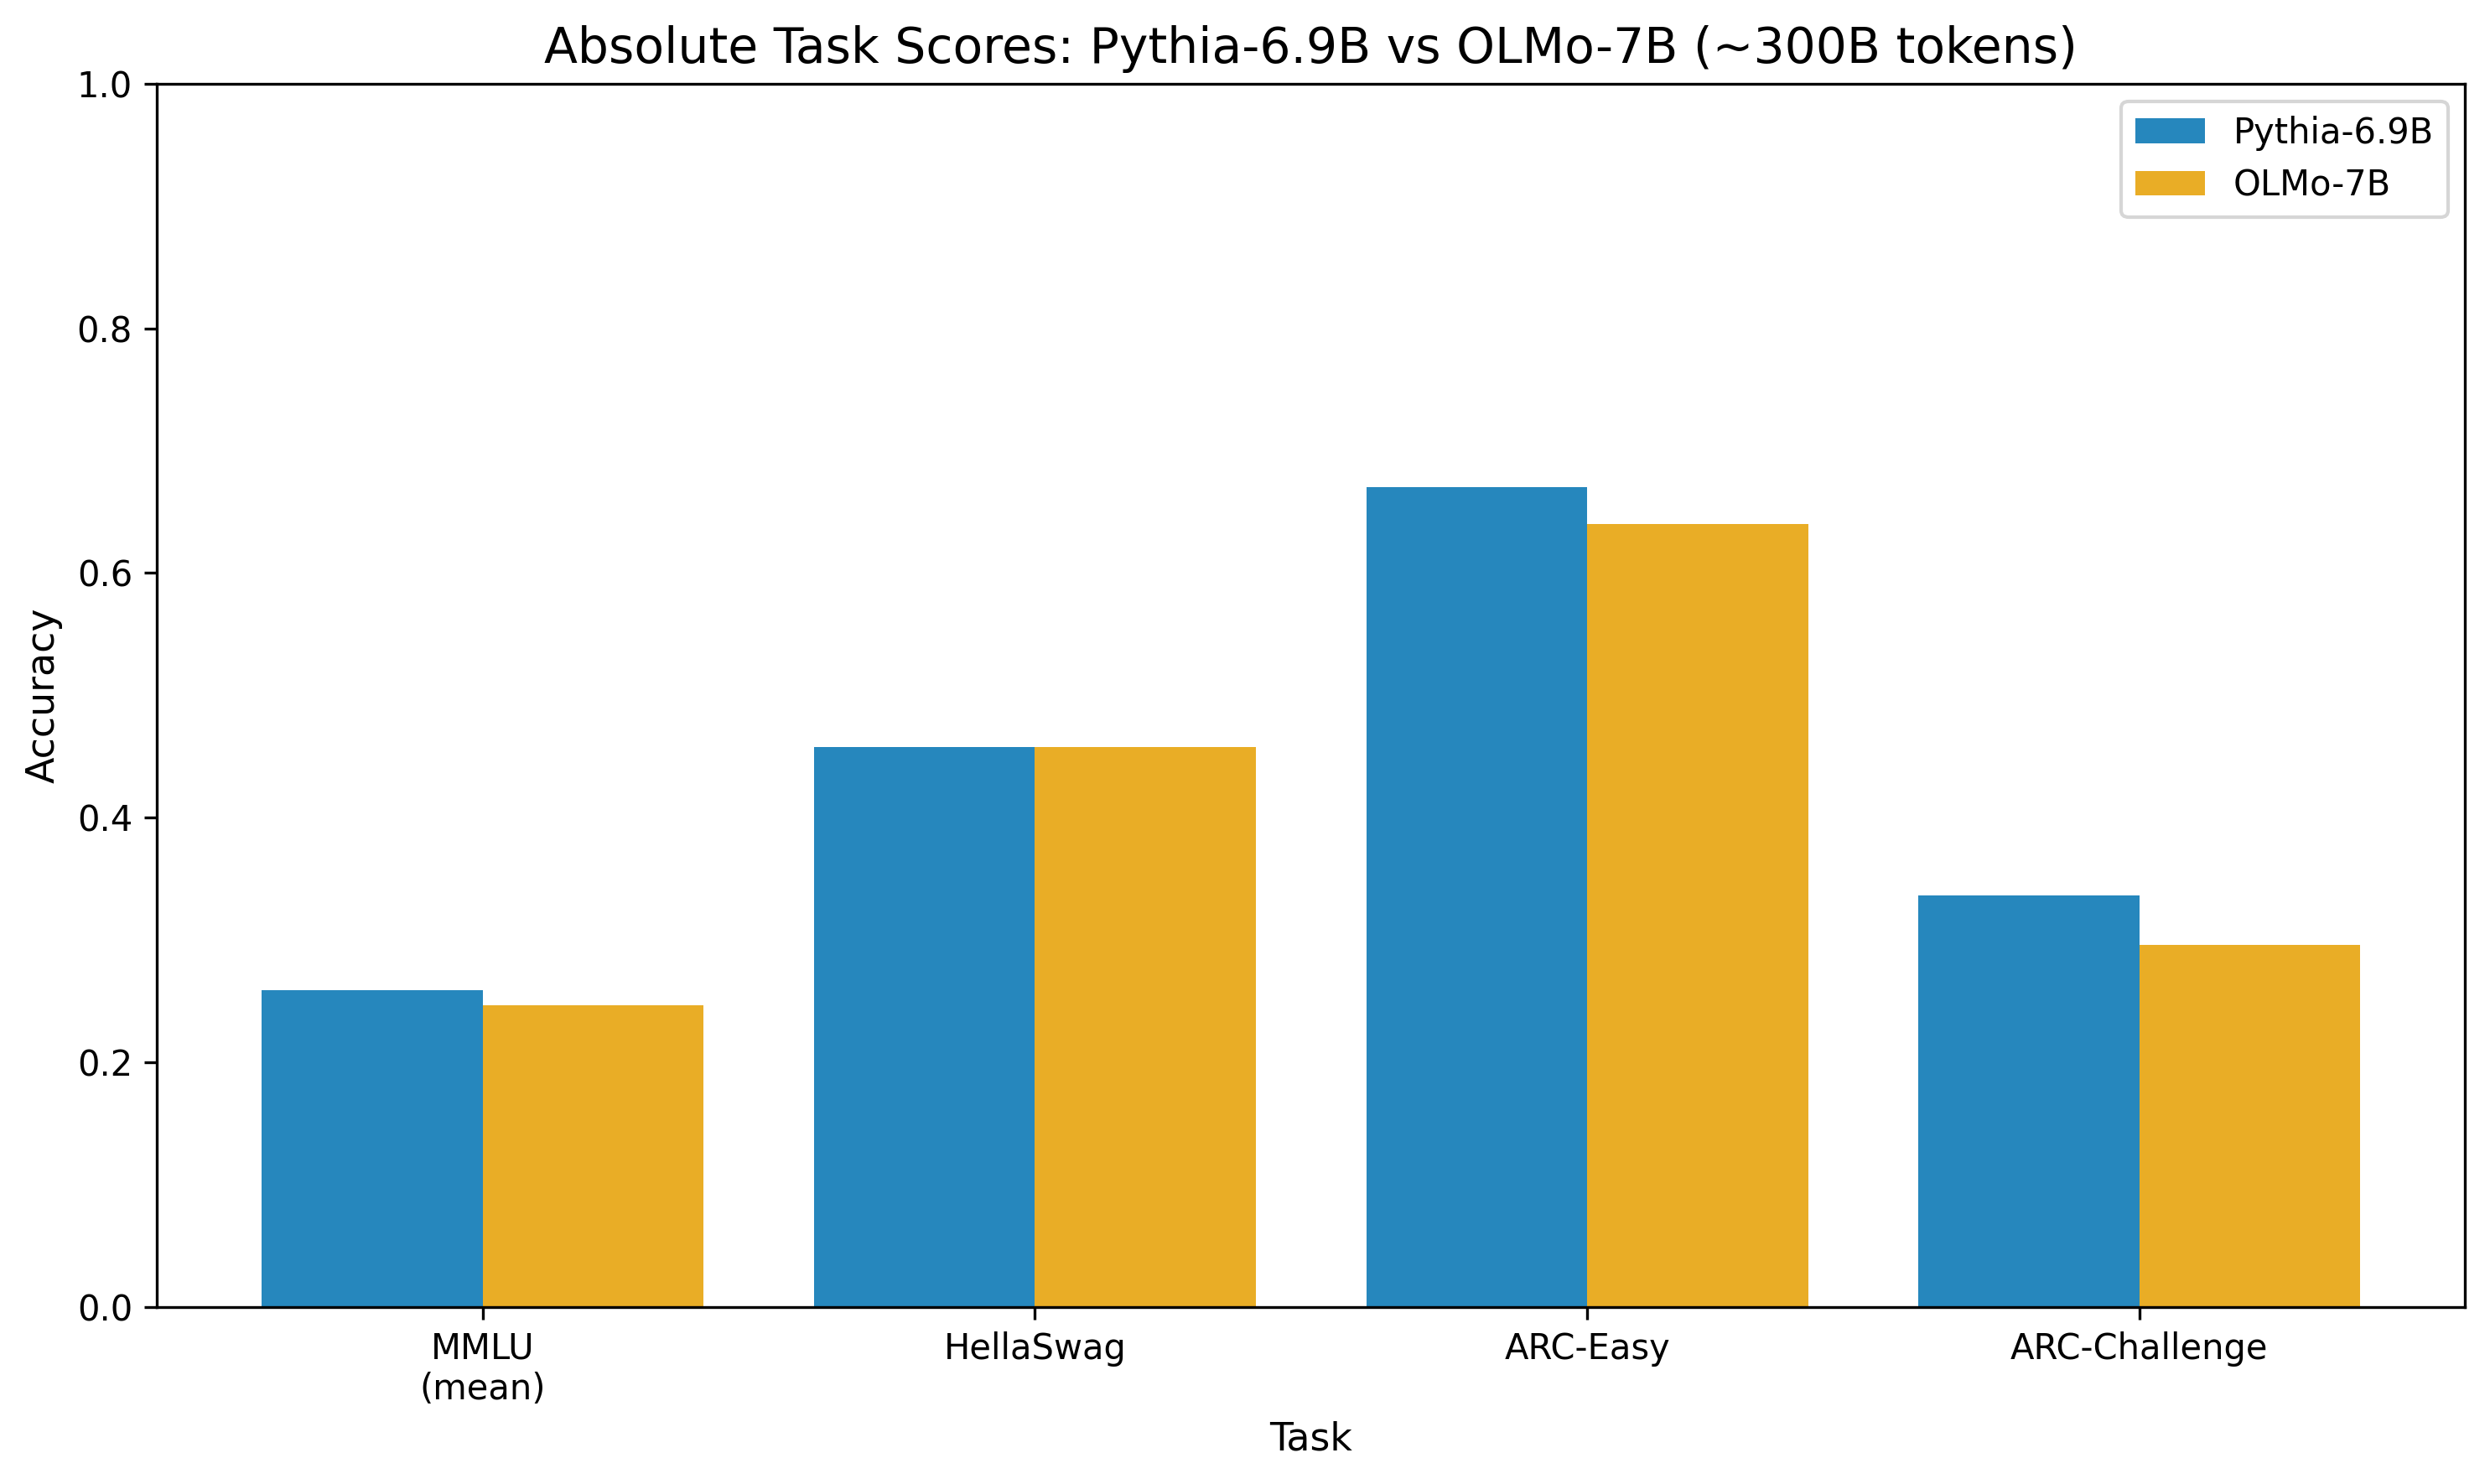
\includegraphics[width=0.48\textwidth]{figures/absolute_scores.png}
\caption{All four benchmark scores for Pythia-6.9B and OLMo-7B at $\sim$300B training tokens.}
\label{fig:scores}
\end{figure}

This convergence has two implications. First, it is consistent with HellaSwag saturation for 6--8B parameter models at $\sim$300B training tokens: web-sourced commonsense knowledge may be largely acquired before this scale, making HellaSwag insensitive to corpus quality differences at this point on the training curve. Second, it collapses the ratio metric into a simple MMLU proxy: $R = \text{MMLU} / 0.458$, meaning ratio differences reflect only MMLU differences, which are themselves architecture-confounded. The generalization balance metric provides no additional signal beyond MMLU alone under these conditions.

\subsection{Analysis: Per-Subject MMLU Heatmap and Contamination Assessment}

\begin{figure}[h]
\centering
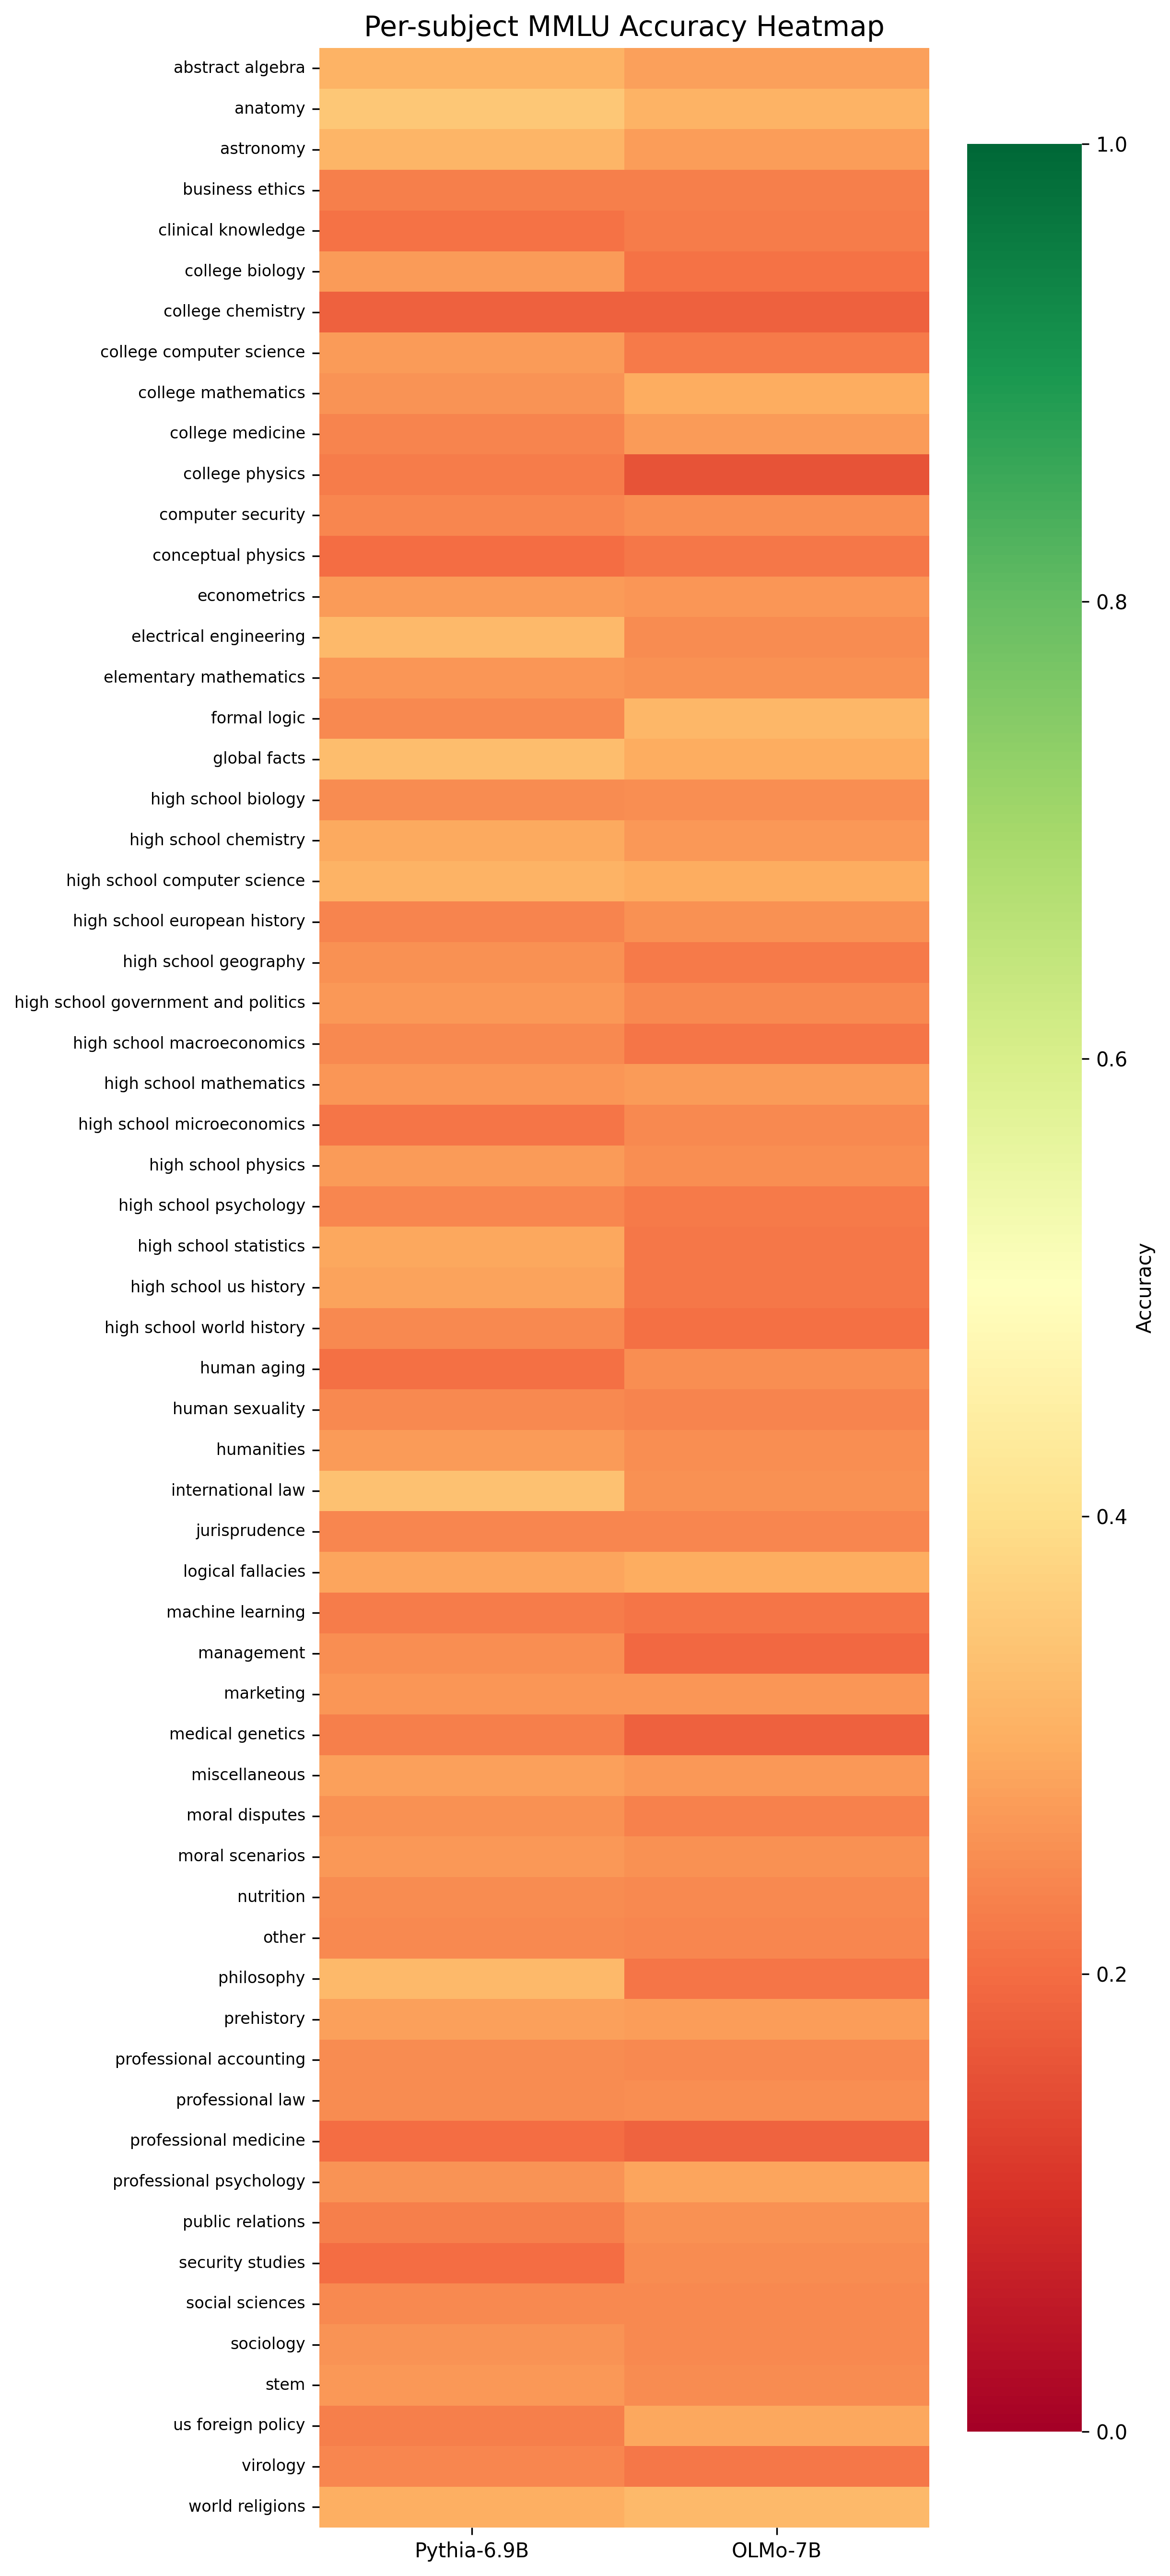
\includegraphics[width=0.9\textwidth]{figures/mmlu_heatmap.png}
\caption{Per-subject MMLU accuracy heatmap across all 57 subjects.}
\label{fig:heatmap}
\end{figure}

Per-subject MMLU accuracy (Figure~\ref{fig:heatmap}) reveals heterogeneous performance patterns. Pythia-6.9B achieves higher accuracy on several STEM subjects, while OLMo-7B achieves higher accuracy on subjects that may overlap with its academic corpus inclusions (S2ORC, Wikipedia). Subjects where OLMo substantially outperforms Pythia include those with strong Wikipedia coverage, which is consistent with Dolma's explicit Wikipedia inclusion but does not rule out contamination. We flag this as a low-to-medium plausibility alternative explanation; definitive contamination assessment would require n-gram overlap analysis between Dolma and MMLU questions, which is outside the scope of this study.

\subsection{Statistical Robustness: Bootstrap Distribution}

\begin{figure}[h]
\centering
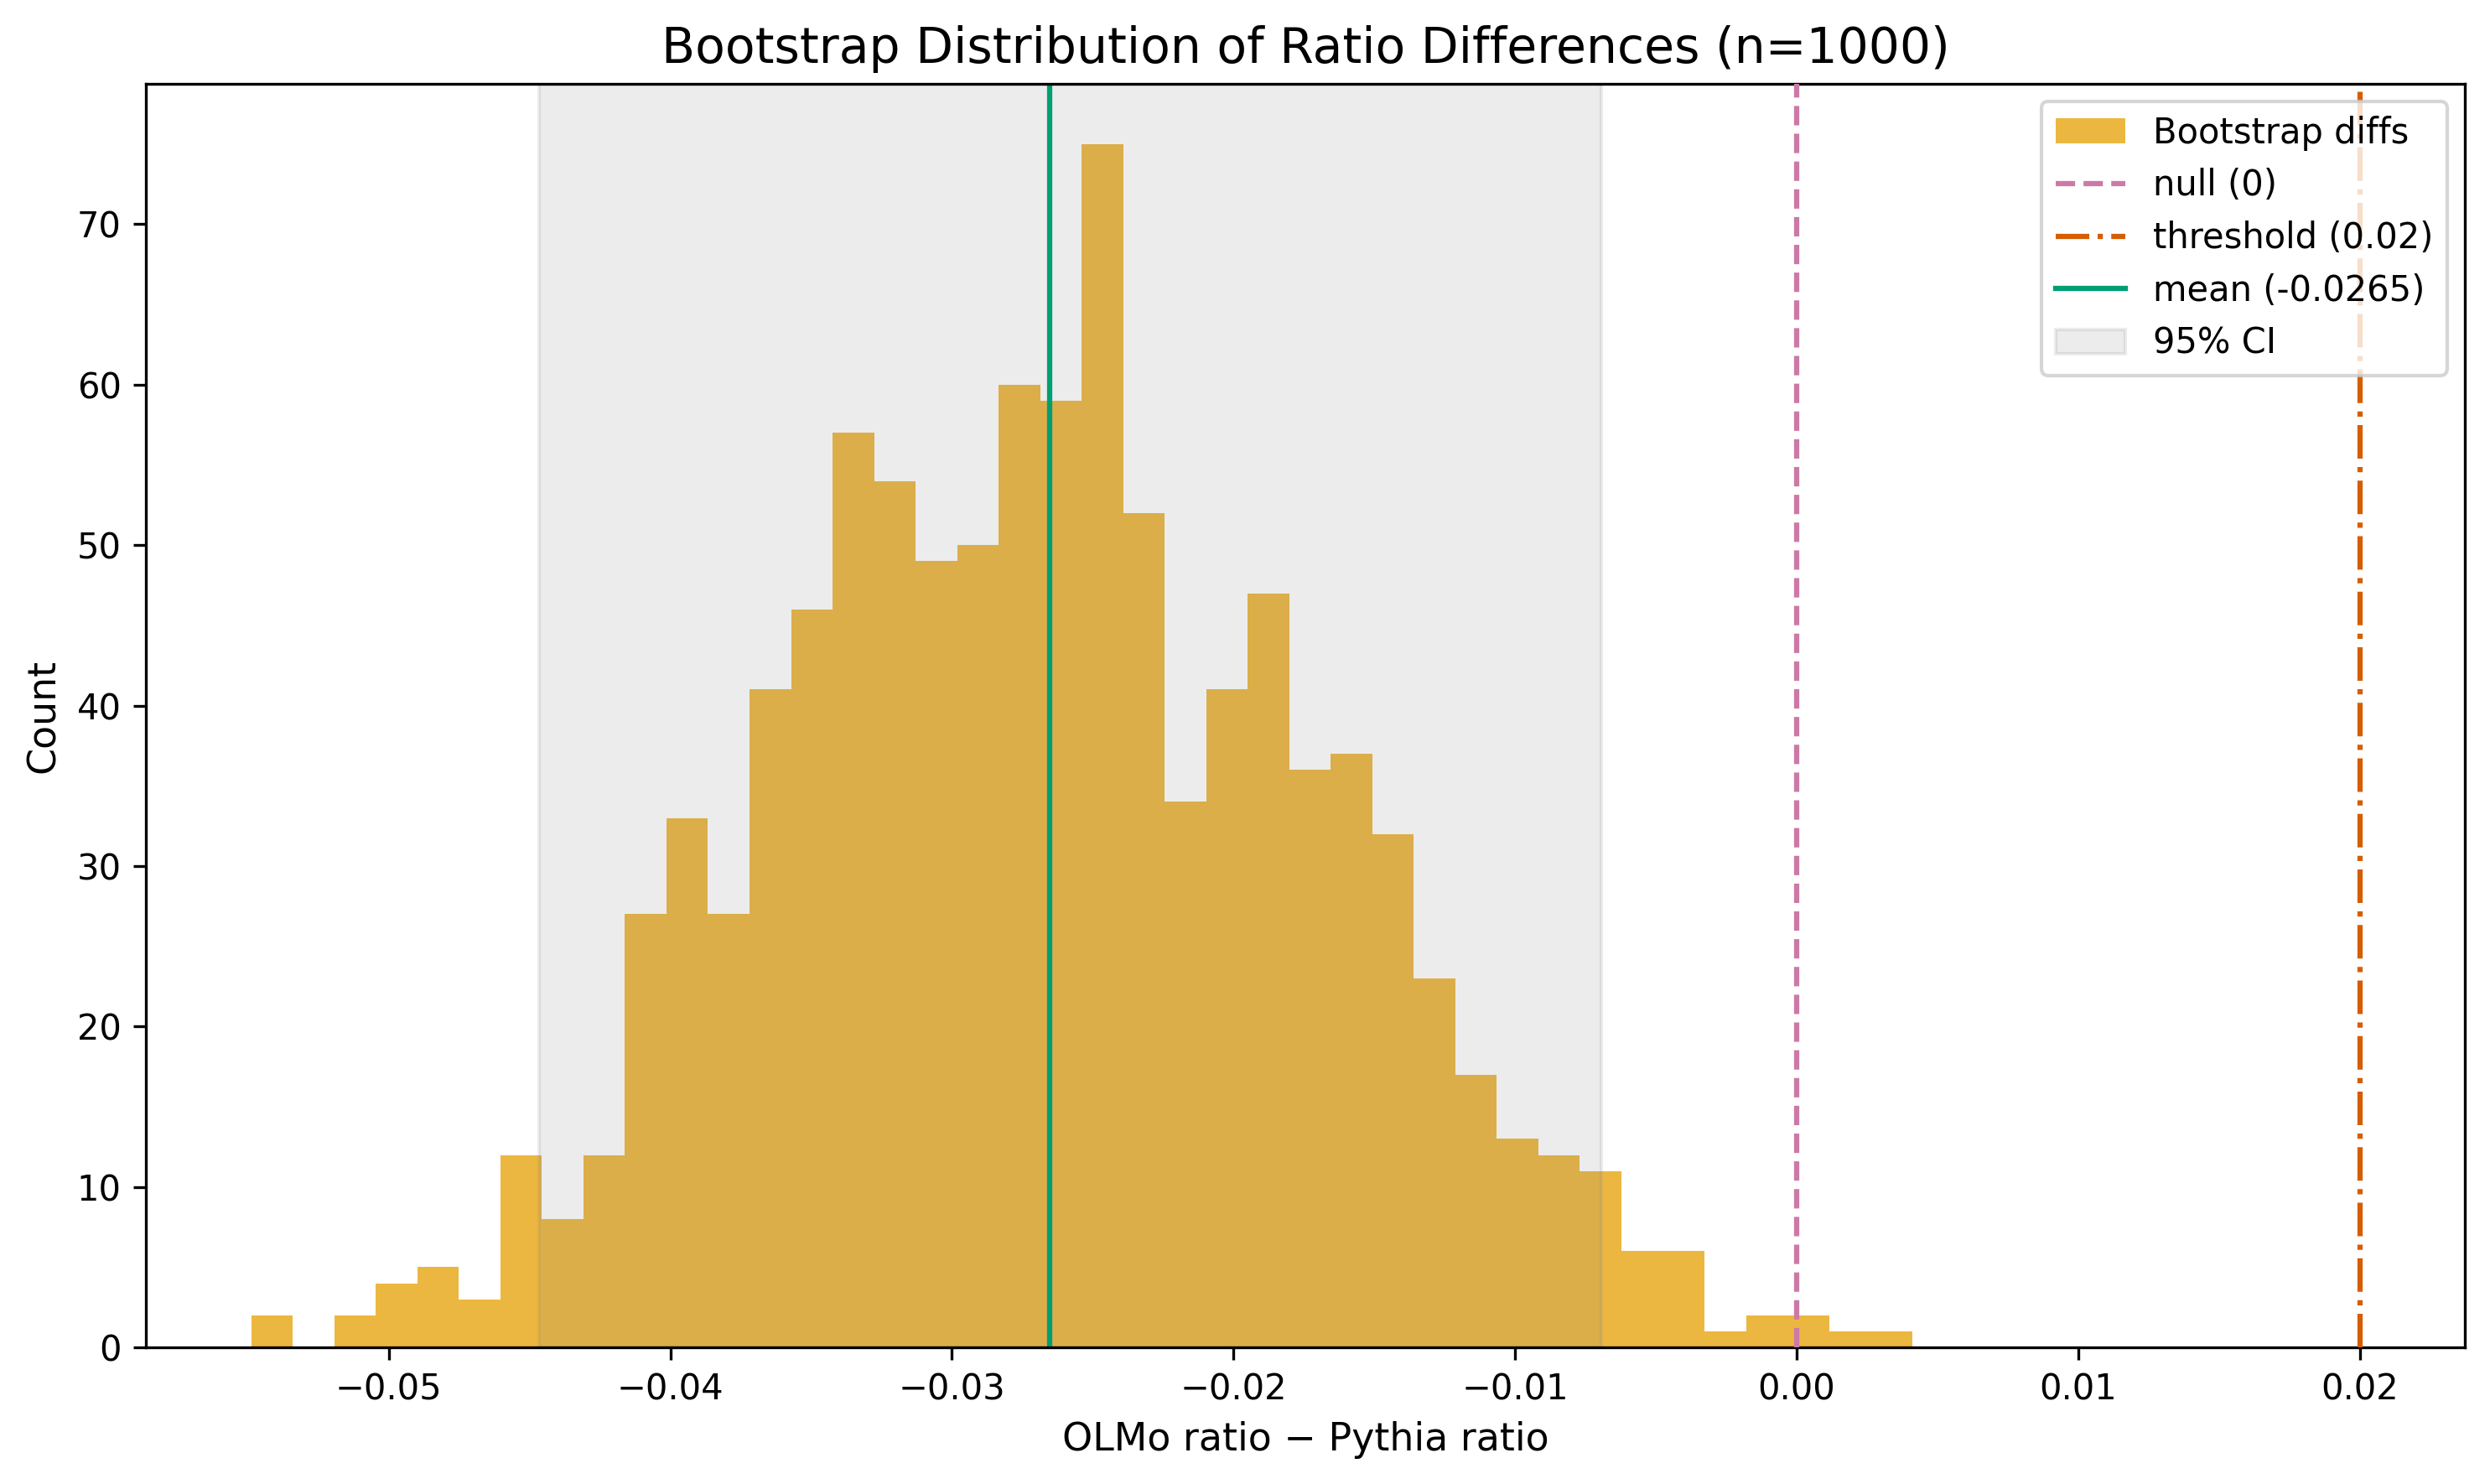
\includegraphics[width=0.48\textwidth]{figures/bootstrap_dist.png}
\caption{Bootstrap distribution of ratio differences (OLMo $-$ Pythia) across 1000 iterations. Neither the null (0, dashed) nor hypothesis threshold ($+$0.02, dotted) falls within the distribution.}
\label{fig:bootstrap}
\end{figure}

The bootstrap distribution (Figure~\ref{fig:bootstrap}) is tightly concentrated below zero. Neither the null value (0) nor the hypothesis threshold ($+0.02$) falls within the 95\% CI. The distribution is approximately symmetric with no heavy tail toward positive values, indicating that the observed reversal is not an artifact of sampling variance.

\subsection{Summary of Results}

\textbf{RQ1} (corpus quality hypothesis): Refuted. Pythia-6.9B achieves a higher MMLU/HellaSwag ratio (0.565 vs.\ 0.538; CI $[-0.045, -0.007]$; Cohen's $d = -2.732$).

\textbf{RQ2} (ARC difficulty delta): Not diagnostic. OLMo achieves higher ARC scores overall; delta difference is small ($-0.012$) and architecture-confounded.

\textbf{RQ3} (HellaSwag denominator informativeness): Denominator is not informative. Exact HellaSwag convergence (0.4580 each) indicates saturation, collapsing the ratio metric to a MMLU proxy.
